% AER-Article.tex for AEA last revised 22 June 2011
\documentclass[AER,draftmode]{AEA}

% The mathtime package uses a Times font instead of Computer Modern.
% Uncomment the line below if you wish to use the mathtime package:
%\usepackage[cmbold]{mathtime}
% Note that miktex, by default, configures the mathtime package to use commercial fonts
% which you may not have. If you would like to use mathtime but you are seeing error
% messages about missing fonts (mtex.pfb, mtsy.pfb, or rmtmi.pfb) then please see
% the technical support document at http://www.aeaweb.org/templates/technical_support.pdf
% for instructions on fixing this problem.

% Note: you may use either harvard or natbib (but not both) to provide a wider
% variety of citation commands than latex supports natively. See below.

% Uncomment the next line to use the natbib package with bibtex 
\usepackage{natbib}

% Uncomment the next line to use the harvard package with bibtex
%\usepackage[abbr]{harvard}
\usepackage{xcolor}
\usepackage{booktabs}
\usepackage{pdflscape}
\usepackage{geometry}
\usepackage{amsmath}
\usepackage{amssymb}
\usepackage{graphicx}
\usepackage{hyperref}
\usepackage{adjustbox}


\usepackage[para,flushleft]{threeparttable}
\usepackage[labelsep = period]{caption}
%\usepackage[hidelinks]{hyperref} %probably nicer option in print (and comment out hypersetup)
\hypersetup{
    colorlinks,
    linkcolor={red!50!black},
    citecolor={blue!50!black},
    urlcolor={blue!80!black}
}

% This command determines the leading (vertical space between lines) in draft mode
% with 1.5 corresponding to "double" spacing.
\draftSpacing{1.5}

% New definitions
\def\sym#1{\ifmmode^{#1}\else\(^{#1}\)\fi}

\begin{document}

\title{Employment and Turnover Effects of the German National Minimum Wage: A Sectoral Analysis}
\shortTitle{Employment Effects of the German NMW}
\author{Dirk Czarnitzki and Helena Kreuter and Jesse Wursten\thanks{Czarnitzki: Centre for European Economic Research (ZEW), Mannheim, Germany. Kreuter: IMT School for Advanced Studies, Lucca, Italy. Wursten: KU Leuven, Naamsestraat 69, 3000 Leuven, Belgium (email: jesse.wursten@kuleuven.be). The authors gratefully acknowledges financial support of the Research Foundation Flanders (FWO) under grant number 1125818N.}}
\date{\today}
\pubMonth{}
\pubYear{}
\JEL{J38, D22}
\Keywords{minimum wage, labour policy, employment elasticity, German national minimum wage, matching estimators, firm level data}

\begin{abstract}
Germany introduced a national minimum wage of €8.50 in 2015. We compare firms in affected sectors to those in unaffected ones using proprietary firm level data. We match on past employment and forward looking creditratings and find only very small negative employment effects (0.014\% of overall employment, ~20 000 jobs lost) and positive effects on turnover in local service sectors. Given Germany's highly developed economy, we believe these results are of interest to the wider, US-centric, minimum wage debate.
\end{abstract}


\maketitle
\section{Introduction} \label{chap:introduction}
The desirability of minimum wage policy has been a heavily debated subject for over a century. On one hand, setting a wage floor can ensure that those who work earn enough to live decently, if not comfortably \citep{Macrosty1898}. On the other, fixing the price of labour might unbalance supply and demand, leading to increased unemployment and the poverty risks that entails. There is still no consensus on the existence or size of this disemployment effect despite hundreds of papers already published on the subject, mainly based on the state-level variation in the US.

The introduction of a national minimum wage in Germany (Jan 1st 2015, €8.50/hr) is a welcome opportunity to obtain a fresh angle on the issue. As a major industrial economy, Germany is more comparable to other western economies than say, Indonesia \citep{Pratomo2016}. The minimum wage introduced is also considerable, exceeding hourly wages in the restaurant and fastfood sector for over 50\% of its employees.\footnote{Own calculations based on the German Socio-Economic Panel.} At 48\% of the median wage, it is similar to long established minimum wages in neighbouring countries.\footnote{Source: OECD} Unlike US studies, we are not limited to geography-level data, but can instead analyse firms directly thanks to our access to the nationally representative, firm level, database of Germany's largest credit rating agency.

The national character of the new minimum wage means the panel approaches standard in the literature cannot be applied (e.g. \citet{Neumark1992, Allegretto2013, Dube2010}). Instead, we exploit differences in pre-treatment wage levels across sectors to identify the effect minimum wages have on employment and turnover levels. We link firms in heavily affected sectors to those in \emph{de facto} unaffected sectors, matching on past employment paths and forward looking creditratings. We surround the matching period by two testing periods (2010-2011 and 2013-2014) to evaluate our matching process.

Our results indicate employment barely responded to the minimum wage introduction. Even among micro firms in East Germany, we only found a reduction in employment growth of 1.8 percentage points. Overall, employment growth in the East of treated firms was 0.8 pp lower than in the control group, in the West the point estimate is indistinguishable from zero. In headcounts, this equates to just 21 482 jobs lost, or 0.05\% of total employment.

Our results are largely in line with other evaluation studies. For example, \citet{Caliendo2018le}, exploiting regional differences in the bite of the minimum wages, find a reduction in overall employment of 0.5\%, concentrated amongst mini-jobbers.\footnote{The mini-job statute in Germany significantly reduces social security contributions for (very) low earning employees.} \citet{Garloff2016} takes this approach one step further by creating region-age-gender cells, each with specific minimum wage bites and employment evolutions. They also finds no meaningful overall employment effect, only a shift from mini jobs to regular employment. Turning to survey data, \citet{Bossler2016} find that employment grew by 1.9\% less in firms which reported employing employees earning less than €8.50/hr in the the IAB Establishment Panel. Relative to total employment that represents a reduction of about 0.15\%.

This study ties in to the wider international debate on the welfare effects of minimum wages and discussion on which mechanisms could explain the lack of employment effects found in some studies (e.g. \citet{Cengiz2018, Allegretto2013, Dube2016a}) but not in others (e.g. \citet{Neumark1992, Liu2016, Neumark2014a}). Our estimates suggest that a part of the cost shock is absorbed by higher turnover, either through firms raising prices or wealthier consumers leading to more product demand. This corroborates existing studies in the US (\citet{Aaronson2001, Allegretto2018}) and Hungary (\citet{Cengiz2018}). Credit ratings remain largely unaffected which indicates firm profit was not meaningfully impacted, this contrasts with \citet{Draca2011}, who find that the national minimum wage introduced in the UK in 1999 lowered profitability of affected firms by 2.7\%. %Expand further on this?  
%\section{Related Literature} \label{chap:literature}
% Overview + Neumark & Wascher
There are essentially three strands in the international minimum wage literature. There are the US-based studies which find strong negative employment effects from the minimum wage, there are US-based studies which find no such effects and then there is literature about the rest of the world. The first, which sees minimum wages as potentially very harmful in developed economies is centered around the \citet{Neumark1992} study. They compare US states over time using (mainly) standard twoway fixed effects models and find that a 10\% increase in the minimum wage lead to a reduction in teen employment of 2-3\%, which is in line with findings from earlier time series models \citep{Brown82}. 

% Card & Krueger
The second strand does not find any disemployment effects and tries to uncover how firms cope with the increases in cost due to the minimum wage. The most notable example is \citet{Card1994}, who conducted surveys in fastfood restaurants in Pennsylvania and New Jersey before and after the NJ minimum wage was increased. Contrary to expectations, they found an \emph{increase} in employment in NJ relative to PA. Additionally, they note that prices in NJ increased more, suggesting restaurants were able to pass through their cost increase to customers.

% DLR & ADR
More recently, \citet{Dube2010} generalised this approach by comparing all counties across state border with a minimum wage differential. They find no statistically significant employment effect in either direction although their standard errors are quite large.\footnote{That is, the mean estimate is 0.016, but at 95\% confidence, they cannot rule out employment elasticities down to -0.178.} \citet{Allegretto2011} come to the same conclusion when they add state-specific time trends to traditional twoway fixed effects specification, or when they restrict the analysis to comparisons within census divisions. 

% Channels of adjustment (prices)
Prices also remain a likely pressure relief valve. \citet{Aaronson2001} use official Bureau of Labor Statistics panel data to show that restaurants respond to minimum wage hikes by increasing their prices one-to-one relative to costs. \citet{Allegretto2018} instead analyse a single high-impact event and find that restaurants in San Jose, CA increased their prices similarly after the 25\% hike in the minimum wage. Other channels of adjustment include pay compression \citep{Hirsch2015} and cost savings through reduced employee turnover \citep{Dube2016a}. 

% International literature
These two strands frequently clash, to the extent that e.g. the ILR Review occasionally asks both sides to submit comments (most recently, \citet{Neumark2017} and \citet{Allegretto2017}). The non-US literature is tied less strongly to the overall debate. \citet{Neumark2006} dutifully provides an overview of minimum wage studies across the world, but quite tellingly, none of them feature in the two ILR Review papers, which reflect the current state of the art. There are many studies based on non-western economies (e.g. Indonesia [\citet{Comola2011}, \citet{Yamada2016}]; Brazil [\citet{Lemos2009}]; China [\citet{Long2016}]; Mexico [\citet{Feliciano1998}]), which are meaningful to the type of country analysed, but are only of limited use to policymakers in western nations. The only two countries which currently feature in the US-based debate are Canada (e.g. tbd) and the United Kingdom (e.g. \citet{Machin2003}, \citet{Metcalf2008}), as they have the right combination of similarity to the US, data availability and particularly variation in the minimum wage.

% German literature
Since its introduction of a national minimum wage on January 1st 2015, Germany should be added to this select list. It is the fourth largest economy in the world, with a high standard of publicly or privately available datasets and a meaningful minimum wage shock, affecting one in five employees nationwide (and up to 65\% in certain sectors). 
\section{Data and Institutional Context} \label{chap:data}
\subsection{Institutional Context}
Western Germany has a long tradition of collective bargaining systems, which kept wages relatively high until the 90's. However, the reunification with  deindustrialised Eastern Germany and the Hartz labor market reforms of 2003 strongly reduced industry compliance, dropping coverage rates from a near universal 85\% in 1990 to barely 60\% in 2013 (and not even 50\% in the East) \citep{Weinkopf2015}. Trade unions, which initially favoured sector-level agreements, started pushing for a national minimum wage, but met heavy political resistance. At the time, Germany was still considered the \emph{sick man of Europe}, with unemployment rates above 10\%, only turning into an economic superstar from 2008 onwards \citep{Dustmann2014}. The surge in economic prowess also led to increased support for a national minimum wage, as rising GDP failed to lift wages for the bottom deciles.

The Social Democratic Party of Germany (SPD) forced the issue in 2013 by making their entry in the governing coalition conditional on the introduction of a national minimum wage \citep{Weinkopf2015}. The Minimum Wage Act went into force on January 1st 2015, setting a national wage floor of €8.50 (then \$11.05) and strengthening collective agreements (exceeding the national minimum). There are only very few exceptions - mainly interns (in a clear educational context), minors, trainees, volunteers and previously long-term unemployed during their first six months in a new job. Additionally, certain sectors (e.g. meat processing, hair dressing) were allowed a two year transition period. We exclude those from our analysis. 

% Replication: ctrl+F #mwtomedianwageGraph
\begin{figure}[htb]
    \centering
    \caption{Ratio of Minimum Wage to Median Wage}
    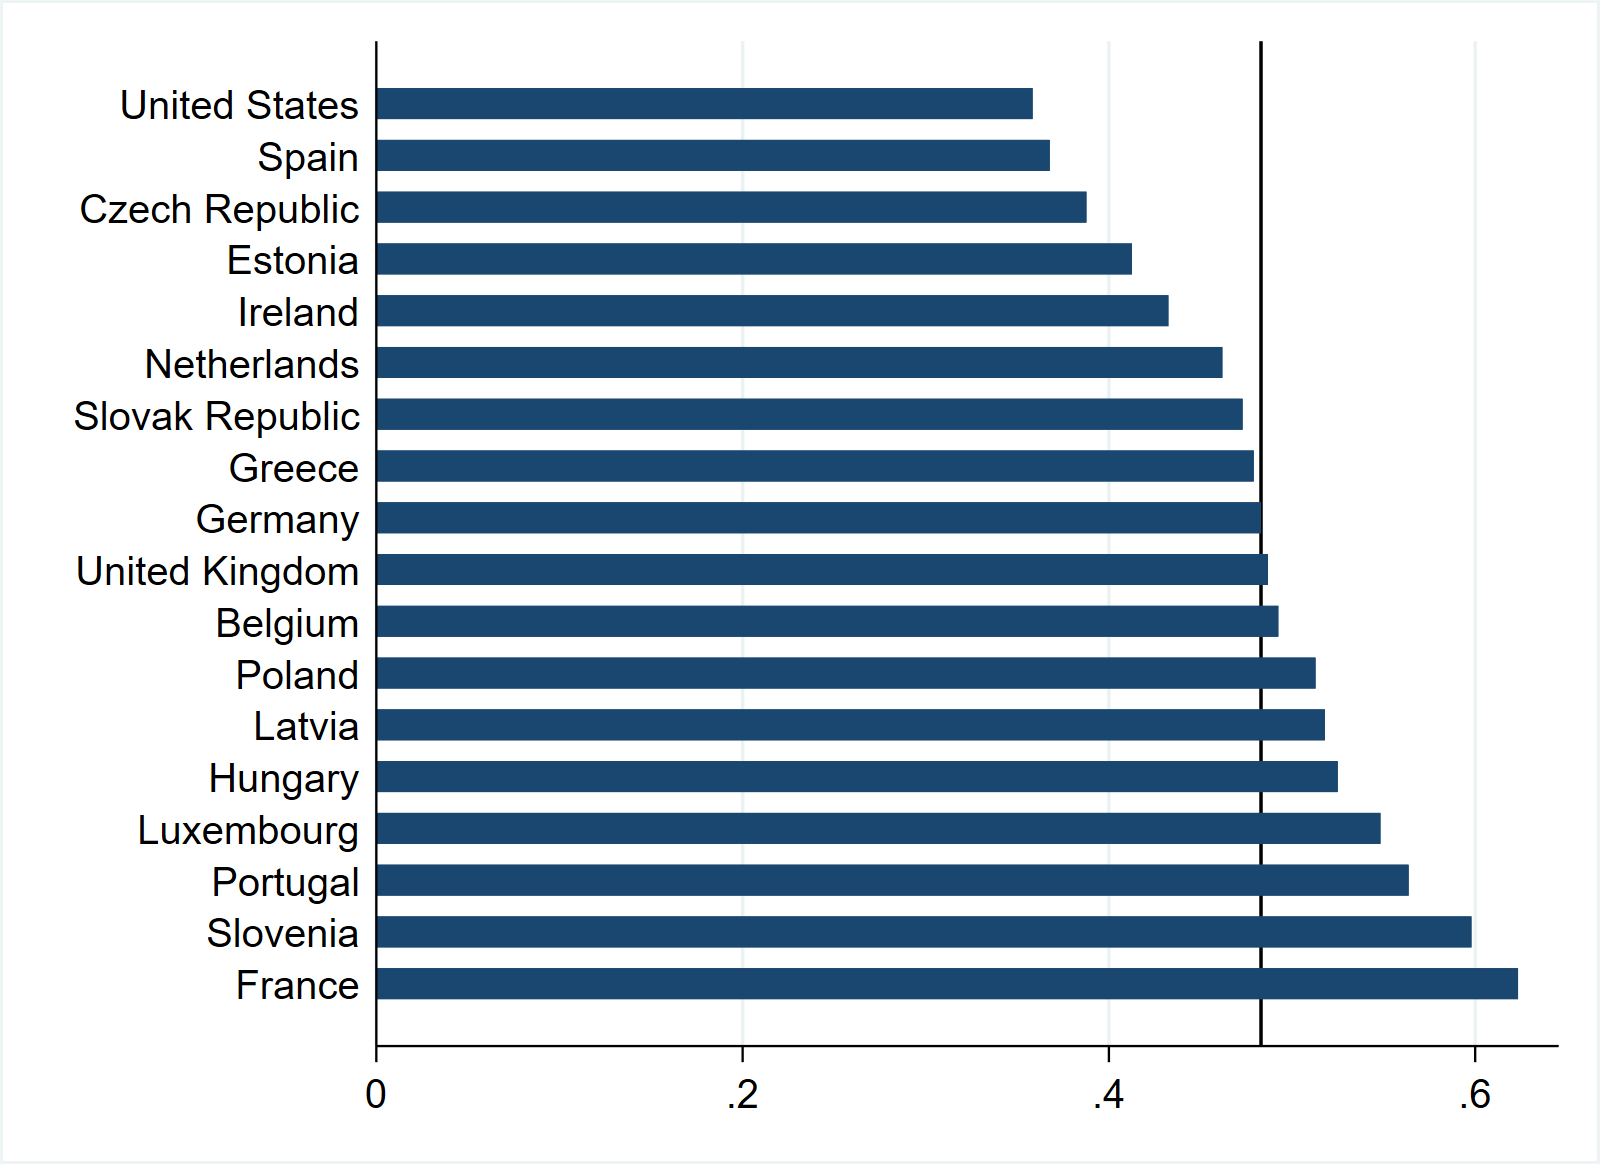
\includegraphics[width=0.60\paperwidth]{Images/mwToMedianWage.png}
    \label{fig:mwtomedian}
    \caption*{Source: \citet{OECDmw}}
\end{figure}

Figure \ref{fig:mwtomedian} shows Germany's National Minimum Wage (NMW) is set at a similar (relative) level as those present in other countries. About 2.8 million eligible employees earned less than €8.50 per hour in 2014 (11\%, \citet{Burauel2017}), albeit with sizeable differences across sectors and regions (Figure \ref{fig:correlationIndicators} in the Appendix). Own back of the envelope calculations based on the SOEP suggest that on average they would require a raise of €2.41/hr to comply with the NMW. Full compliance would raise the total wage bill by 2\%.

The minimum wage commission decides on the future evolution of the policy and consists of voting representatives from industry (3), unions (3) and two advisory members from the academic community. This led to a first increase in 2017, when the minimum wage was raised from €8.50 to €8.84, suggesting the minimum wage will be raised gradually (the 2017 hike amounts to a 4\% increase), rather than in larger discrete jumps as is more customary in the US.\footnote{The average size of minimum wage changes in the US between 1990-2013 was 9.5\% \citep{Wursten2017}.}

\subsection{Firm-level Data}
The core of this study is the Mannheim Enterprise Panel (MUP) hosted by the Centre for Economic Research (ZEW). It is based on data obtained from Creditreform, the largest creditrating agency in Germany and covers all German corporations \citep{Steven2017}. The dataset is representative for the German economy and can thus be used to formulate population-level conclusions \citep{Bersch2014}. The main variables of interest are employment and turnover, but also the assigned creditratings. These are based on a combination of public and private sources, e.g. public trade registers and court filings as well as private data on payment reliability and even manager interviews. As a result, these ratings contain more information on a firm's health than traditional balance sheet items. We drop outliers based on changes in the creditrating and employment or turnover (depending on the dependent variable) to retain the largest and smallest firms but still filter out input errors as well as massive swings due to mergers and acquisitions.

\subsection{Sector-level Treatment Indicator}
Our identification strategy is based on comparing firms in heavily affected sectors to similar counterparts in largely unaffected sectors. In order to construct this `vulnerability' indicator, we turn to the German Socio-Economic Panel (SOEP version 32), a yearly survey of private households which has been conducted since 1984 in West Germany and since 1990 in East Germany (comparable to the Current Population Survey in the US). Crucially, it contains monthly wages as well as hours worked information, which we combine to obtain an estimate of each individual's hourly wage. Restricting our sample to eligible persons in 2013-2014 (right before the introduction of the minimum wage), we can then calculate for each two-digit sector how many employees were earning less than the NMW.\footnote{We use the Nace Rev 2 classification, which is based on the international ISIC standard and can fairly easily be compared to the US NAICS system.} Given the substantial wage differences between East and West Germany, we further split this across the two parts. 

Table \ref{table:sectorBite} provides an overview of the most and least affected sectors. As in the US, we see that the restaurant and fastfood sector (Nace 56) is most heavily affected. Unaffected sectors are for example waste collection, financial services and the higher value manufacturing sectors. The table also shows the average gap between the sub-NMW earners' wage in 2014 and the NMW and how much that sector's total wage bill would rise under full compliance (and no other wage movement).

We use the share of sub-NMW workers to split the industries into three groups: treated, grey zone and controls, for East and West Germany separately given their economic differences. Any sector where this share exceeds 30\% is defined as treated, below 10\% is considered control. Those in between we consider to be in the grey zone and exclude from the analysis. Table \ref{table:sectorOverview} shows the treatment allocation per sector-region (region: East or West Germany), as well as the distribution of firms in our regression sample over sector-regions. The differences between East and West Germany are remarkably stark. Only the food and beverages sector (`restaurants') and accommodation sectors are treated in the West, whereas only seven sectors qualify as controls in the East. Conversely, there are 29 treated sectors in the East, whereas the West has 27 control sectors. 

% Replication: ctrl+F #sectorOverviewTable
\begin{table}[htbp]\centering
\setlength\tabcolsep{3pt}
\small
\caption{Treated, Untreated and Greyzone Sectors}\label{table:sectorOverview}
\begin{threeparttable}
    \begin{tabular}{r|c|c|l}
    \toprule
Nace & Treatment & \# of firms & Nace  \\
Code & West-East & West-East & Text\\
\midrule
56&	T-T&	1018 - 124&	Food and beverage service activities\\
55&	T-T&	626 - 158&	Accommodation\\
\midrule
47&	GZ-T&	9149 - 1255&	Retail trade, excl. of motor vehicles and motorcycles\\
70&	GZ-T&	6270 - 313&	Activities of head offices; management consultancy activities\\
45&	GZ-T&	4646 - 1017&	Wholesale and retail trade and repair of motor vehicles and motorcycles\\
68&	GZ-T&	4066 - 605&	Real estate activities\\
71&	GZ-T&	2702 - 454&	Architectural and engineering activities; technical testing and analysis\\
52&	GZ-T&	2021 - 309&	Warehousing and support activities for transportation\\
82&	GZ-T&	1670 - 169&	Admin, office support and other business support activities\\
66&	GZ-T&	1509 - 160&	Activities auxiliary to financial services and insurance activities\\
10&	GZ-T&	1233 - 257&	Manufacture of food products\\
77&	GZ-T&	968 - 236&	Rental and leasing activities\\
23&	GZ-T&	881 - 202&	Manufacture of other non-metallic mineral products\\
73&	GZ-T&	987 - 68&	Advertising and market research\\
69&	GZ-T&	874 - 99&	Legal and accounting activities\\
79&	GZ-T&	763 - 81&	Travel agency, tour operator and related activities\\
74&	GZ-T&	746 - 51&	Other professional, scientific and technical activities\\
31&	GZ-T&	625 - 89&	Manufacture of furniture\\
93&	GZ-T&	506 - 65&	Sports activities and amusement and recreation activities\\
13&	GZ-T&	352 - 72&	Manufacture of textiles\\
78&	GZ-T&	317 - 31&	Employment activities\\
11&	GZ-T&	272 - 29&	Manufacture of beverages\\
95&	GZ-T&	215 - 44&	Repair of computers and personal and household goods\\
14&	GZ-T&	171 - 18&	Manufacture of wearing apparel\\
80&	GZ-T&	130 - 21&	Security and investigation activities\\
63&	GZ-T&	118 - 8&	Information service activities\\
15&	GZ-T&	68 - 10&	Manufacture of leather and related products\\
50&	GZ-T&	53 - 5&	Water transport\\
12&	GZ-T&	11 - 1&	Manufacture of tobacco products\\
\midrule
64&	C-C&	956 - 51&	Financial service activities, excl. insurance and pension funding\\
38&	C-C&	608 - 219&	Waste collection, treatment and disposal activities; materials recovery\\
35&	C-C&	652 - 167&	Electricity, gas, steam and air conditioning supply\\
37&	C-C&	108 - 34&	Sewerage\\
84&	C-C&	106 - 18&	Public administration and defence; compulsory social security\\
39&	C-C&	37 - 4&	Remediation activities and other waste management services\\
\midrule
43&	C-GZ&	15765 - 3844&	Specialised construction activities\\
25&	C-GZ&	4969 - 964&	Manufacture of fabricated metal products, excl. machinery and equipment\\
41&	C-GZ&	3159 - 772&	Construction of buildings\\
28&	C-GZ&	3102 - 392&	Manufacture of machinery and equipment n.e.c.\\
62&	C-GZ&	2603 - 250&	Computer programming, consultancy and related activities\\
26&	C-GZ&	1180 - 170&	Manufacture of computer, electronic and optical products\\
42&	C-GZ&	796 - 297&	Civil engineering\\
27&	C-GZ&	898 - 144&	Manufacture of electrical equipment\\
32&	C-GZ&	834 - 110&	Other manufacturing\\
20&	C-GZ&	594 - 86&	Manufacture of chemicals and chemical products\\
85&	GZ-C&	536 - 95&	Education\\
33&	C-GZ&	464 - 124&	Repair and installation of machinery and equipment\\
24&	C-GZ&	498 - 71&	Manufacture of basic metals\\
29&	C-GZ&	339 - 68&	Manufacture of motor vehicles, trailers and semi-trailers\\
17&	C-GZ&	329 - 49&	Manufacture of paper and paper products\\
30&	C-GZ&	135 - 32&	Manufacture of other transport equipment\\
21&	C-GZ&	124 - 19&	Manufacture of basic pharmaceutical products and preparations\\
65&	C-GZ&	105 - 4&	(re-)Insurance and pension funding, excl. compulsory social security\\
36&	C-GZ&	36 - 21&	Water collection, treatment and supply\\
51&	C-GZ&	18 - 0&	Air transport\\
9&	C-GZ&	6 - 3&	Mining support service activities\\
6&	C-GZ&	3 - 0&	Extraction of crude petroleum and natural gas\\
    \bottomrule
    \end{tabular}
\begin{tablenotes}
\item \footnotesize T: treated, C: control, GZ: grey zone (excluded). Table sorted by treatment status and number of firms in the sector. Unlisted sectors are a) in grey zone in both areas, b) excluded based on legislative reasons or c) excluded due to pre-existing higher sectoral minimum wage agreements.
\end{tablenotes}
\end{threeparttable}
\end{table}
%\section{<optional extra chapter>} \label{chap:spatialheterogeneity}

% Example equations
\begin{align}
    y_{it} &= \alpha + \beta x_{it} + \delta mw_{it} + \epsilon_{it} \label{eq:pols} \\
    y_{it} &= \alpha_i + \theta_t + \beta x_{it} + \delta mw_{it} + \epsilon_{it} \label{eq:2fe} \\
    y_{it} &= \alpha_i + \theta_t + \gamma_s * t + \beta x_{it} + \delta mw_{it} + \epsilon_{it} \label{eq:timeTrends}
\end{align}

%\section{Estimation Strategy} \label{chap:estimation}
<Optional econometrics chapter[TD]>
\section{Estimation} \label{chap:results}
% Matching procedure (test change)
Based on the treatment/control assignment described in Section \ref{chap:data}, we match treated to control firms based on their previous employment and credit rating patterns. The outcome of interest is the mean difference in log employment evolutions from 2014-2015 and 2014-2016 between the two groups (semi-elasticity of employment w.r.t. the minimum wage). We apply large-sample bias correction and use AI standard errors, which factor in matching uncertainty \citep{Abadie2003,Abadie2006}.

% Covariate imbalance
Table (?) shows why the matching procedure is required. In particular, the second to last column shows that there are substantial differences between the treated and control sectors in their employment patterns and credit ratings. These differences are not constant over time, indicating that analyses which do not take this into account risk picking up this trend rather than a causal effect of the minimum wage introduction, particularly given that we expect the minimum wage effect to be small in size. The final column shows that our matching procedure deals with this issue quite effectively, ensuring that we are comparing firms that are on a similar growth trajectory (past employment) and are assumed to have similar prospects (credit ratings). Similarities in the mean might still mask differences along the rest of the distribution. In Figure \ref{fig:sumStats}, we show that the distribution of the six matching variables is very similar for the treated (solid line) and matched (dotted) observations. The same cannot be said for the raw controls (dashed), where especially for employment we observe considerable differences in densities.

\begin{figure}[htbp]
    \centering
    \caption{Distribution of the matching variables}
    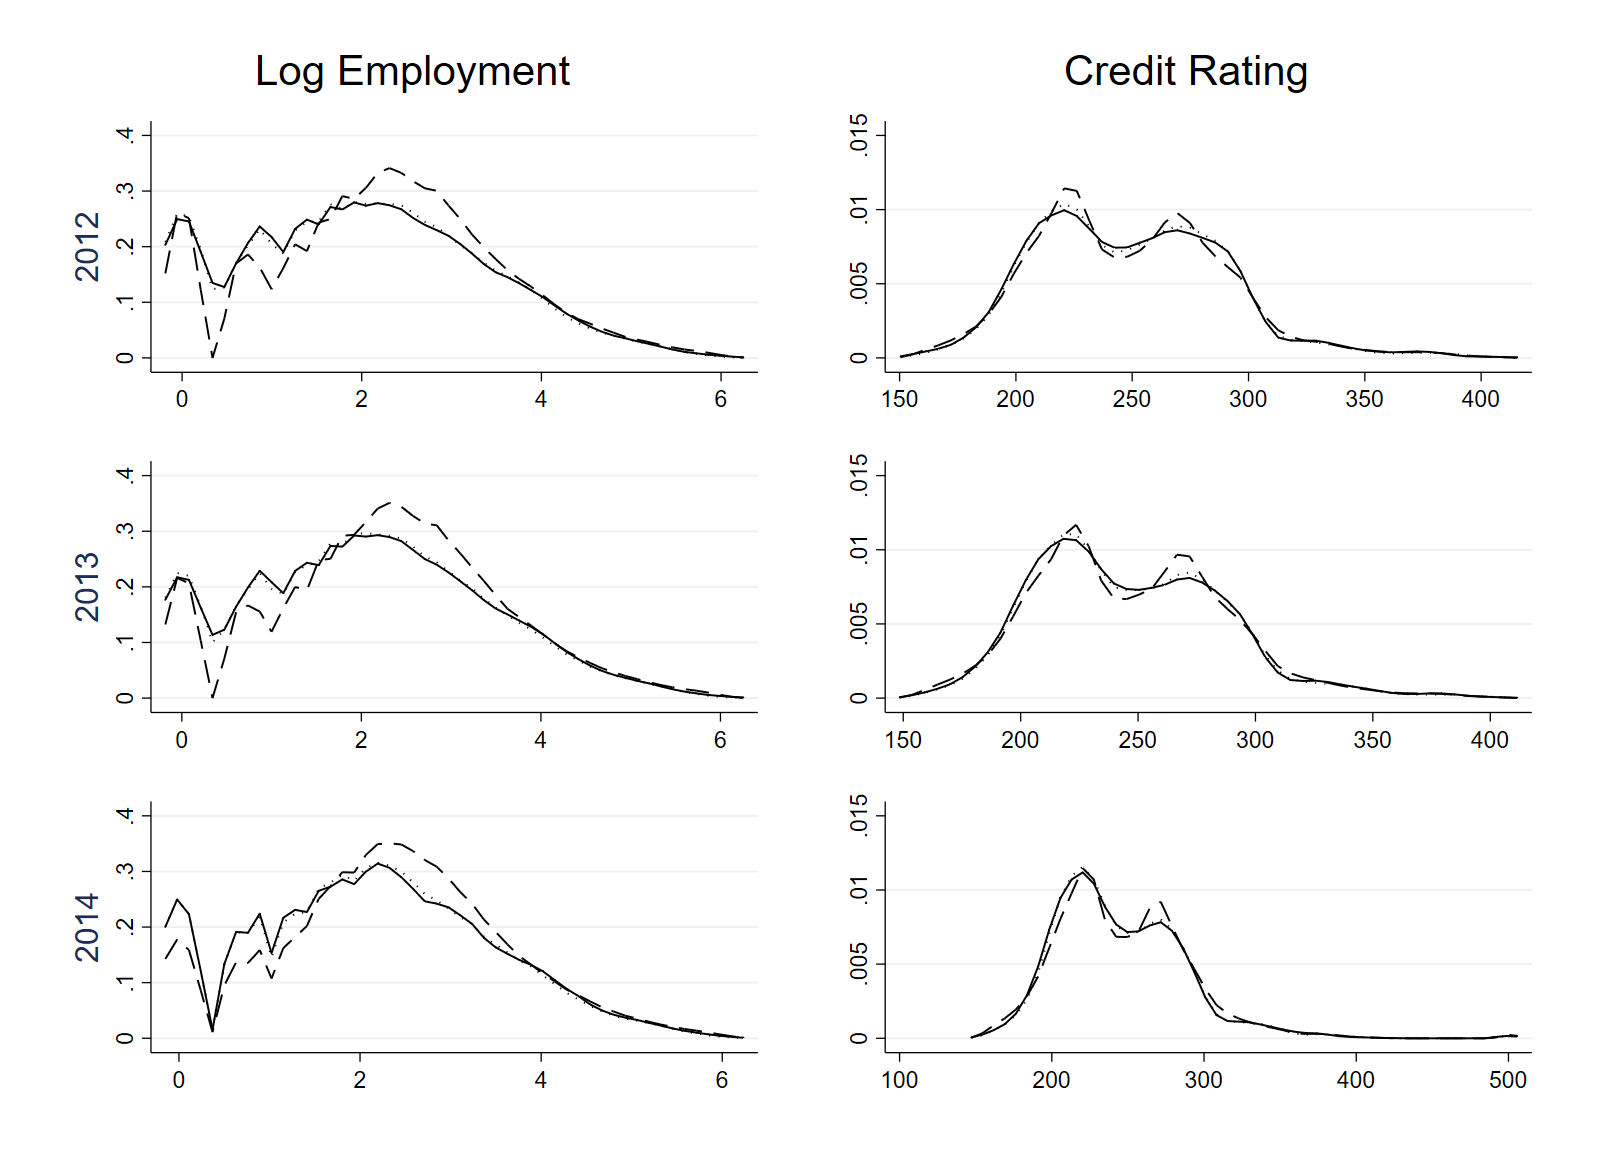
\includegraphics[width=0.70\paperwidth]{Images/summaryStats_graphs.png}
    \label{fig:sumStats}
    \caption*{Solid line: density of the treated observations. Dashed line: density of the full set of control observations. Dotted line: density of the matched set of control observations.}
\end{figure}
% Reference year/OLS
Table \ref{table:mainResults} shows the main results under different scenario's. Columns (1) and (2) provide estimates from a simple OLS regression where we include the matching variables as predictor. We have two years of post-intervention data and have chosen to use 2014 as reference point for both. That is, instead of comparing 14-15 and then 15-16, both are expressed relative to 2014. In the end, we are interested in the effect of the treatment, not necessarily whether there is a significant difference between 15 and 16.\footnote{The sample is restricted to be identical in both years.} As a result, the estimates represent the full effect up to that year and should not be added together.

% Main Results
% Replication: ctrl+F #mainResultsTable
\begin{table}[htbp]\centering
\caption{Employment and Turnover Effects}\label{table:mainResults}
\begin{threeparttable}
\begin{tabular}{l|cc|cc}
\toprule
&\multicolumn{2}{c|}{East}&\multicolumn{2}{c}{West}\\
&Emp&Turn & Emp&Turn\\
&(1)&(2)&(3)&(4)\\
\midrule
$\Delta$ Growth 14-15 &-.005& -.001& .002 & .011\\
&(.002)\sym{**}& (.004)& (.004) & (.006)\sym{**} \\
$\Delta$ Growth 14-16 &-.008& -.003& .001 & .033\\
&(.003)\sym{**}& (.006)& (.006) & (.009)\sym{***} \\
\midrule
\# of treated &5654& 3981& 1562 & 1115\\
\# of controls &39012& 27787& 39012 & 27788\\
\# of controls used &8008& 2876& 2699 & 1090\\
\midrule
SDM 13-14 &.02& -.01& .02& .02\\
Level Diff 2013&0& -.01& .01& 0\\
Trend 2011-2014&\checkmark&\checkmark&\checkmark&\checkmark \\
Specification & Base & U & Base & Prod $+$ U\\
\bottomrule
\end{tabular}
\begin{tablenotes}
\item $\Delta$ Growth is the difference in growth between the treated and control. SDM refers to the standardised difference in means. 
Level Diff 2013 indicates the difference in log levels between treated and control in 2013. 
Trend indicates how this level difference evolved between 2011 and 2014.
Specification shows which matching specification scored best at the evaluation criteria. Prod: match also on 2014 labour productivity of firm (emp/turn),
U: ... on the unemployment rate within state.
\item Matching uncertainty robust AI standard errors in parentheses \citep{Abadie2006}.
\item \emph{Stars}: \sym{*} \(p<0.1\), \sym{**} \(p<0.05\), \sym{***} \(p<0.01\)
\end{tablenotes}
\end{threeparttable}
\end{table}

% Size Results
% Replication: ctrl+F #sizeResultsTable
\begin{table}[htbp]\centering
\caption{Employment and Turnover Effects - Micro and Small Enterprises}\label{table:sizeResults}
\begin{threeparttable}
\begin{tabular}{l|cccc|cccc}
\toprule
&\multicolumn{4}{c|}{East}&\multicolumn{4}{c}{West}\\
&\multicolumn{2}{c}{Micro}&\multicolumn{2}{c|}{Small}&\multicolumn{2}{c}{Micro}&\multicolumn{2}{c}{Small}\\
&Emp&Turn & Emp&Turn&Emp&Turn & Emp&Turn\\
&(1)&(2)&(3)&(4)&(5)&(6)&(7)&(8)\\
\midrule
$\Delta$ Growth 14-15 &-.009& -.006&.002& -.005& -.002 & .026& .019 & .016\\
&(.004)\sym{**}& (.005)&(.003)& (.005)& (.008) & (.01)\sym{***}& (.006)\sym{***} & (.009)\sym{*} \\
$\Delta$ Growth 14-16 &-.018& .003&-.001& -.008& -.007 & .046& .034 & .043\\
&(.006)\sym{***}& (.008)&(.005)& (.008)& (.011) & (.018)\sym{**}& (.009)\sym{***} & (.013)\sym{***} \\
\midrule
\# of treated &2875& 1821&2091& 1401& 552 & 342& 665 & 457\\
\# of controls &39009& 27785&39012& 27787& 39009 & 27787& 38908 & 27788\\
\# of controls used &3001& 1579&2534& 1283& 512 & 328& 610 & 471\\
\midrule
SDM 13-14 &-.02& -.01&.09& -.01& -.01& -.01& .02& .03\\
Level Diff 2013&-.27& -.27&.01& .02& -2.4& -.08& .16& .02\\
Trend 2011-2014&\checkmark&\checkmark& $\times$&\checkmark&?&$\times$&\checkmark&? \\
Specification & MJ & MJ & Base & Base & MJ & Prod $+$ U&Prod $+$ U&Base\\
\bottomrule
\end{tabular}
\begin{tablenotes}
\item $\Delta$ Growth is the difference in growth between the treated and control. SDM refers to the standardised difference in means. 
Level Diff 2013 indicates the difference in log levels between treated and control in 2013. 
Trend indicates how this level difference evolved between 2011 and 2014.
Specification shows which matching specification scored best at the evaluation criteria. Prod: match also on 2014 labour productivity of firm (emp/turn),
U: ... on the unemployment rate within state.
MJ: ... on the share of mini-jobbers within state.
\item Matching uncertainty robust AI standard errors in parentheses \citep{Abadie2006}.
\item \emph{Stars}: \sym{*} \(p<0.1\), \sym{**} \(p<0.05\), \sym{***} \(p<0.01\)
\end{tablenotes}
\end{threeparttable}
\end{table}



% Main Results/OLS
What we find is that there is a statistically significant negative impact overall, but it is relatively small. That is, the introduction of the national minimum wage reduced employment rates in the highly affected sectors by just 1 percent, much less than predicted ex ante (see Section \ref{chap:discussion}). Moreover, this result is not homogeneous across sectors. For example, the OLS results in column (2) suggest that the restaurant and fastfood sector benefited from the new minimum wage, with employment increases of 4\% in 2015, rising to 6\% in 2016.

% Main Results/Why we match (repeat)
However, these results may be driven by pre-existing trends, as well as observable and unobservable differences between firms in the treated and untreated industries. In this non-randomized experiment, there is very little we can do against the latter, but our matching procedure should at least ensure that we are comparing firms with a similar past and in a similar financial situation. 

% Main Results/Matching outcomes
Results are presented in columns (3) and (4). Qualitatively, the results remain the same. I.e. we still estimate a small negative impact overall (-1.1\% in 2016) and a positive one in the restaurant sector. The latter does become about 20\% smaller, suggesting employment in the restaurant sector increased by 3\% in 2015, up to 5\% in 2016. In an alternative specification, we omit the credit ratings and focus on matching pretreatment employment evolutions. The impact on the restaurant sector remains essentially unchanged, with respectively a three and a five percent increase (column 6). The estimated impact across all affected sectors becomes markedly larger, rising to a 1.5\% employment loss by 2016 (column 5).


% Results by firm size (overall)
Table (??) shows results per firm size. Starting with the results across all sectors in columns (1)-(3), we see that the only significant effect is found among the smaller firms (10-49 employees), where we see a drop of 1.6\%.\footnote{The effects are identical for micro firms of less than ten employees.} The effect on medium sized firms (50-249) is smaller (-0.9\%) and only significant at 10\%. Large firms (250+) even appear to have benefited from the minimum wage introduction. However, the estimate is based on just 57 treated and 48 control firms and only significant at 10\%.

In the restaurant sector, a similar pattern can be observed. The only significant effect is found in the micro firms (1-10 employees), where we see an increase of 7.5\% by 2016. The effect remains positive for small firms (1.5\%), but loses significance. Medium sized firms appear unaffected, with very imprecise estimates centered around -1\%. There are insufficient large firms to perform a matching exercise there.

\section{Discussion} \label{chap:discussion}
% Employment in affected sectors in 2014

% Ex ante
% Knabe Schob 2008: -0.84M
% Ragnitz  Thum 2007: -1.1M
% Bachmann 2008: -1.2M
% Bauer 2009: -0.85M
% Muller Steiner 2010: -140K

% Ex post
% Caliendo 2017: -0.3% / 78K in regular, 2.4% / 180K in mini-jobs / regional variation in bite
% Bossler 2016: -1.9% / 60K / survey question on having a worker <MW / parallel trend is questionable
The small but negative overall effect on employment (-1.1\%) is broadly in line with other studies of the German minimum wage. \citet{Bossler2016} finds a reduction in employment of 1.9\% based on the IAB Establishment Panel 2011-2015 which included a question on whether the firm had employees earning less than €8.50. The larger effect size may be due to a cleaner treatment-control distinction, although this comes at the cost of reduced similarity in the pretreatment period, which could also partially drive their result. The approach in \citet{Caliendo2018le} is more similar to ours, but where we get the identifying variation from sectoral differences, they use geographical differences in the minimum wage ``bite''. They find a much smaller effect on regular employment (-0.3\%), but a significantly larger effect for mini-jobbers (-2.9\%).\footnote{Mini jobs are limited to a monthly pay of €450 per month and are tax free, although the employer still has to pay social security contributions.} This differential impact on regular versus marginal employment is also present in \citet{Garloff2016}, who uses region-age-gender variation in the minimum wage bite to identify the employment effect. They find that the number of mini jobs lost balance out the gains in regular employment, suggesting there might be a shift from one form to the other.

In order to compare our results to the numerous ex ante predictions, we first need to convert the relative employment loss to an absolute number of jobs foregone. In 2014, Germany counted 38 million employees.\footnote{Source: Destatis. Includes both regular and marginal employment, but exludes interns and the self-employed.} Of those, 4.8 million were employed in an affected sector. Multiplying this number by our semi-elasticity, our back-of-the-envelope estimate suggests 54 000 jobs were lost due to the national minimum wage. This represents a mere 0.14\% of total employment and is in line with the previously mentioned ex-post studies. It is however far below most ex-ante predictions. Those were generally clustered around a million jobs lost (\citealp{Knabe2008}: 0.84M; \citealp{Ragnitz2007}: 1.1M; \citealp{Bachmann2008}: 1.2M; \citealp{Bauer2009}: 0.85M), with the notable exception of \citet{Muller2010}, who predicted a more conservative 150 000 job losses. A potential explanation for this large discrepancy is that those ex-ante studies were performed at a time when German unemployment was twice as high (10\% vs 5\% in 2014) and estimated wages in the bottom decile were remarkably lower \citep{Muller2013}.

Next to the overall effect, we also find evidence of heterogeneous impacts across sectors, as shown by Figure \ref{fig:sectorSplit}. The bars represent the average treatment effect per sector, split for West and East Germany (resp. dark and light grey). The number of treated firms is shown on the left. Not only are some sectors more strongly affected, a handful appear to have profited from the minimum wage introduction. Most notably, the restaurant and fastfood sector (NACE 56) saw robust (and as shown in Table \ref{table:mainResults}, statistically significant) employment growth after the minimum wage introduction. 

There are multiple potential explanations. Restaurant prices are relatively volatile, changing by 2-3\% each year even in low general inflation periods.\footnote{Source: Destatis, Verbraucherpreisindex.} This makes it easier to pass on cost increases to the consumer without suffering short-term competitive losses. There is some US evidence for this, e.g. \citet{Allegretto2018} show that restaurants in San Jose, CA passed on to costumers nearly the entire cost increase due to a 25\% hike in the local minimum wage. A complementary explanation is the presence of a positive product demand effect if increased earnings are spent on food away from home. Indeed, 2015 saw a 12\% decline in the number of people who \emph{never} eat out as well as an increase in the number of people eating out \emph{often}.\footnote{Source: Statista, \url{https://www.statista.com/statistics/561124/eating-out-frequency-germany/}, accessed April 2018.} This might put the results from American studies in perspective, which are generally limited to studying either restaurants or teenagers.\footnote{Due to the low level of the US minimum wage, no other meaningful sectors employ considerable numbers of potentially affected workers.} If the restaurant sector there can adapt to higher minimum wages in a similar fashion, it can be dangerous to extrapolate the lack of disemployment effects found in that sector (e.g. \citealp{Dube2010}, \citealp{Allegretto2011}) to the wider economy.

\begin{figure}[htbp]
    \centering
    \caption{Average treatment effect by sector (split East/West Germany)}
    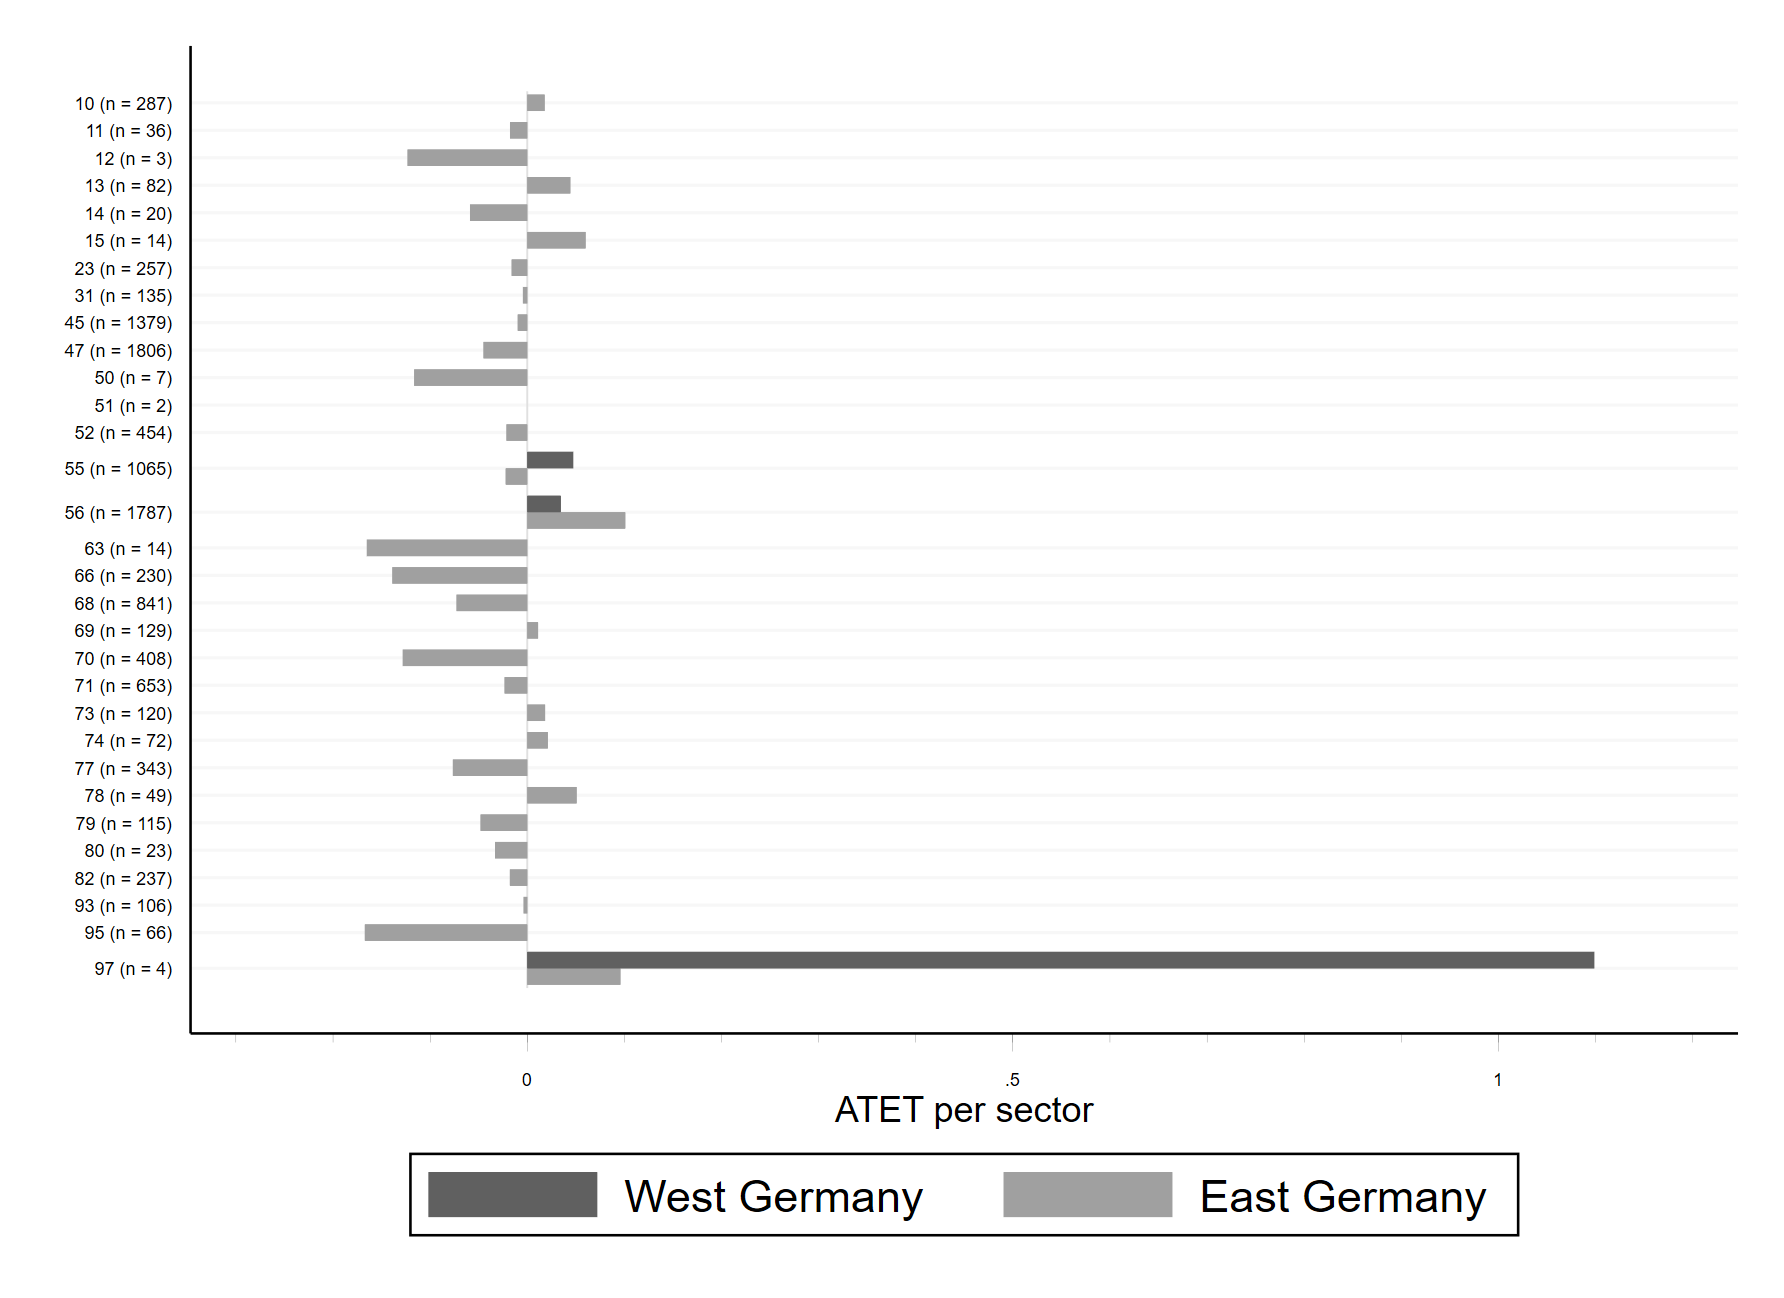
\includegraphics[width=0.70\paperwidth]{Images/ATET_per_sector_graph_ditor.png}
    \label{fig:sectorSplit}
\end{figure}
\section{Robustness Checks} \label{chap:robustness}
Our proprietary firm level dataset allows us to match treated firms directly to non-treated firms, taking into account both their employment trends and their prospective financial situation. This combination of backwards and forwards looking matching variables makes that we can be more confident in our parallel trend assumption than the difference-in-differences approaches commonly applied. Moreover, unlike the geographic aggregate based studies in the US, we can differentiate effects based on firm size. However, in contrast to survey-based data (e.g. the IAB Establishment Panel), we cannot directly identify whether a firm paid any of its employees less than €8.50 per hour. Instead, we assign treatment status based on their sector classification, determining whether sectors are affected based on data from the SOEP, setting thresholds based on economic intuition. In this section, we first test the sensitivity of our results to the choice of these thresholds and then test whether they hold when we add all Italian firms as potential controls.

\subsection{Different thresholds}\label{sec:sectors}
% Robustness Check (Tw)
\begin{table}[htbp]\centering
\caption{Employment effects within Germany, alternative thresholds}\label{table:robustness1}
\begin{tabular}{l|*{2}{c}|*{2}{c}|*{2}{c}}
\toprule
&\multicolumn{2}{c|}{OLS}&\multicolumn{2}{c|}{Baseline}&\multicolumn{2}{c}{Without CR}\\
&All & Resto &All & Resto &All & Resto \\
&(1)&(2)&(3)&(4)&(5)&(6)\\
\midrule
Employment effect & -0.002 & 0.046 & 0.002 & 0.034 & -0.001 & 0.039   \\
2014-15 & (0.002) & (0.009)\sym{***}& (0.003) & (0.011)\sym{***} & (0.002) & (0.009)\sym{***} \\
Employment effect & -0.004 & 0.068 & -0.003 & 0.068 & -0.003 & 0.062   \\
2014-16 & (0.003) & (0.012)\sym{***}& (0.004) & (0.015)\sym{***} & (0.003) & (0.013)\sym{***} \\
\midrule
N&&&&&&\\
\# of treated & 31773 & 2127 & 29532 & 1872 & 31773 & 2127     \\
\# of controls & 96553 & 96553 & 90017 & 90017 & 96553 & 96553    \\
\# of controls used & 84752 & 64600 & 33064 & 4602 & 84752 & 64600       \\
\bottomrule
\multicolumn{7}{p{0.7\textwidth}}{\emph{Stars}: \sym{*} \(p<0.1\), \sym{**} \(p<0.05\), \sym{***} \(p<0.01\)}\\
\end{tabular}
\end{table}


In the baseline results, firms were split into three groups based on the share of employees earning less than €8.50 an hour in 2013-14. The thresholds, at 10 and 30\%, were quite strict to ensure a clear distinction into treated and control. As an alternative, we shift these limits to 15 and 25\%. This should reduce the variance of our estimate (as we have more data), but comes with the risk of introducing attenuation bias as (more) firms will now be assigned to the wrong treatment status.\footnote{Essentially, we introduce measurement error in the treatment variable, which would be our independent variable if we were in a standard regression framework.}

Table \ref{table:robustness1} shows the results with the laxer treatment assignment. Compared to the main results (Table \ref{table:mainResults}), the estimate have become more precise, with standard errors slightly decreasing across the board. The overall coefficient estimates have moved closer to zero, which is consistent with the attenuation bias story, but also highlights the fragility of the negative employment effect, which was small to be begin with. On the contrary, the positive effect in the restaurant sector remains unaffected, indicating that result is not driven by the choice of control firms.

\subsection{Italian control firms}\label{sec:italy}
% Robustness Check (Italy)
% Run 2_Regressions_firmLevel, with the generateTables option set. Uncomment >local italianTable "useItaly == 1"<. Remove middle columns.
\begin{table}[htbp]\centering
\caption{Employment effects with Italian control firms}\label{table:robustness2}
\begin{tabular}{l|*{2}{c}|*{2}{c}}
\toprule
&\multicolumn{2}{c|}{OLS}&\multicolumn{2}{c}{Matching (Without CR)}\\
&All & Resto &All & Resto \\
&(1)&(2)&(3)&(4)\\
\midrule
Employment effect & 0.011 & 0.046 & 0.004 & 0.030   \\
2014-15 & (0.003)\sym{***} & (0.008)\sym{***} & (0.003) & (0.008)\sym{***} \\
Employment effect & 0.028 & 0.094 & 0.016 & 0.066   \\
2014-16 & (0.004)\sym{***} & (0.011)\sym{***} & (0.004)\sym{***} & (0.011)\sym{***} \\
\midrule
N&&&&\\
\# of treated & 11846 & 2030  & 11846 & 2030     \\
\# of controls & 293259 & 293259  & 293259 & 293259    \\
\# of controls used & 227868 & 158006  & 227868 & 158006       \\
\bottomrule
\multicolumn{5}{p{0.7\textwidth}}{\emph{Stars}: \sym{*} \(p<0.1\), \sym{**} \(p<0.05\), \sym{***} \(p<0.01\)}\\
\end{tabular}
\end{table}

In the second robustness check, we swap the donor pool to all Italian firms. Italy did not experience any significant movement in its (sector level) minimum wages in the time period studied and is the fourth largest economy in Europe (after Germany, the UK and France). The Italian data was obtained through AIDA, an oft-used database compiled by Bureau van Dijk. Due to the more demanding accounting requirements in Italy, the database is rather comprehensive, especially with regards to employment numbers and much more so than its German counterpart Dafne. Unfortunately, it does not contain credit ratings, so we are limited to matching on past employment (2012-2014).

As shown in Table (A??) in the appendix there are considerable differences between the treated German firms and the untreated Italian firms. As a result, we do not put much stock in the naive OLS results reported in columns (1) and (2) of Table \ref{table:robustness2} and move straight to the matching estimators in columns (3) and (4). As in the previous robustness check, we notice how fragile the negative overall effect is - now, we even find a significantly positive effect, although the effect size remains small at 1.6\%. The positive effect in the restaurant sector stays robust with coefficient estimates (3\% in 2015, up to 6.6\% in 2016) that are remarkably similar to the previous results despite the completely different set of control firms.
\section{Conclusion} \label{chap:conclusion}
In this paper we present a novel approach to analyse the employment effects of the national German minimum wage introduced on January 1st 2015 and discuss how this policy shock can inform the wider international minimum wage debate, which is particularly active in the US. We start from individual hourly wages to determine which sectors were vulnerable to the new wage floor and which should remain unaffected.\footnote{We exclude the grey zone in between from our analyses.} Then we turn to firm level data and match firms in treated sectors to similar firms in unaffected sectors. The richness of the (proprietary) dataset used allows us to not only match on past employment, but also on the firm's credit score in 2014, which represents expectations about its future.

We find a very small overall effect, suggesting employment in treated firms grew 1.1\% slower than in their untreated counterparts, equivalent to 54 000 jobs lost. Although this result is in line with existing studies \citep{Bossler2016, Caliendo2018le}, we also show that it is rather fragile. For example, changing the thresholds that assign treatment status or adding Italian firms as potential controls already leads to respectively insignificant and minor positive employment effect estimates.

The same cannot be said for our second main result, that the restaurant sector benefited strongly from increased bottom decile earnings across Germany. This finding matters particularly because in the main US-based studies, it is either restaurant or teenage employment that is investigated. If similar mechanisms are at play in the US as in Germany, it would be misleading to extrapolate the restaurant-based employment effects to the rest of the US economy, which may enjoy the same pricing flexibility and product demand effects.

Overall, we can conclude that the catastrophic labour market effects predicted by ex ante studies (over one million job losses) have failed to materialise. Instead, it led to robust wage growth \citep{Bossler2016} and at most very limited employment losses, and that only in particular sectors. In others, most notably the food services sector, the national minimum wage even led to employment growth, suggesting there is a place for minimum wage policy in a social planner's toolbox.



% Remove or comment out the next two lines if you are not using bibtex.
\bibliographystyle{aea}
\bibliography{MW_bib}

\appendix
\appendix
\section{Appendix}
\subsection{Matching Procedure Justification}
The treatment effect after matching can be calculated as in Equation \ref{eq:1te}, where $\hat{\alpha}$ is the estimated treatment effect, $T$ is the set of treated observations, $C$ that of the controls. $Y_{it}$ is the outcome value of interest for observation $i$ at time $t$. $w_j$ is the weight assigned to each control observation. In matching without replacement and without ties this would be either one or zero. In matching with replacement and or ties this can be any real value larger than zero. These weights sum up to the number of treated observations.
\begin{equation} \label{eq:1te}
    \hat{\alpha} = \sum_{i \in T} \Delta Y_{i, 15} - \sum_{j \in C} w_j \Delta Y_{j,15}
\end{equation}

In line with synthetic control method studies (e.g. \citealp{Abadie2006, Dube2015}), we assume $Y_{it}$ can be modeled in a multi factor error structure (see e.g. \citealp{Chudik2015, Bai2009}) as in Equation \ref{eq:2mfs}. $\alpha_i$ is the firm-specific treatment effect, $D_t$ is one from 2015 onwards and zero before, I(..) indicates whether the firm is treated. $c_i$ is a firm-specific fixed effect, $\delta_t$ is a period specific common shock and $\epsilon_{it}$ is a mean zero (time-varying) idiosyncratic shock. $F_t$ is a time-varying economy wide shock that affects each firm differently, according to their specific factor loading $\lambda_i$. There can be a potentially large number of these, but for ease of exposition we stick to one.

\begin{equation}\label{eq:2mfs}
    Y_{it} = \alpha_i D_t I(i \in T) + c_i + \delta_t + F_t \lambda_i + \epsilon_{it}
\end{equation}

Substituting in our model for $Y_it$ and expanding the difference operator leads to Equation \ref{eq:3fullte}.

\begin{equation}\label{eq:3fullte}
    \begin{split}
         \hat{\alpha} =\sum_{i \in T} \alpha_i + &(c_i - c_i) + (\delta_{15} - \delta_{14}) + \lambda_i * (F_{15} - F_{14}) + (\epsilon_{i,15} - \epsilon_{i,14})  \\
         - \sum_{j \in C} w_j [ &(c_j - c_j) + (\delta_{15} - \delta_{14}) + \lambda_j * (F_{15} - F_{14}) + (\epsilon_{j,15} - \epsilon_{j,14})]
    \end{split}
\end{equation}

The $c$'s drop out due to the time differing. Given that $\sum_{i \ in T}1 = \sum_{j \in C} w_j$, the deltas in treated and control also cancel out eachother. The $\epsilon$'s are assumed to be mean zero, so as $T$ and $C$ get large, these also drop out, leaving us with Equation \ref{eq:4reducedte}.

\begin{align}\label{eq:4reducedte}
         \hat{\alpha} &=\sum_{i \in T} \alpha_i + \lambda_i * (F_{15} - F_{14}) 
         - \sum_{j \in C} w_j \lambda_j * (F_{15} - F_{14}) \nonumber\\
                     &=\sum_{i \in T} \alpha_i + \bigg(\sum_{i \in T}\lambda_i - \sum_{j \in C} w_j \lambda_j\bigg) * (F_{15} - F_{14})
\end{align}

The remaining bias terms are a function of the disparity in the treated and untreated factor loadings $\lambda$. This is where the synthetic control method intuition comes in: if we match on pretreatment outcome values, then as $T$, $C$ and the number of pretreatment periods we match on get larger, the average difference between treated and untreated factor loadings $\lambda$ goes to zero. The idea is that with just one pretreatment period you might still be able to find a set of weights $w_j$ such that treated and untreated firms with different factor loadings match due to compensating idiosyncratic $\epsilon$'s. As the pretreatment period becomes longer, this becomes increasingly unlikely (given time constant weights). Instead, this only remains possible if your matching algorithm achieved matches by picking controls firms such that the weighted sum of their factor loadings $\sum_{j \in C} w_j \lambda_j$ equals the sum of the treated factor loadings $\sum_{i \in T}\lambda_i$. Under that assumption, Equation \ref{eq:4reducedte} reduces to Equation \ref{eq:5success}, where all bias terms have been accounted for.

\begin{equation}\label{eq:5success}
    \hat{\alpha} = \sum_{i \in T}\alpha_i
\end{equation}


% Replication: ctrl+F #sectorBiteTable
\begin{table}[htbp]\centering
%\setlength\tabcolsep{3pt}
\tiny
\caption{Overview of bite, gap and wage bill indicators by sector (East-West)}\label{table:sectorBite}
\begin{threeparttable}
    \begin{tabular}{r|c|c|c|l}
    \toprule
Nace & Share    & Gap       & Wage Bill     & Nace  \\
Code & West-East& West-East & West-East     & Text \\
\midrule
55&	52 - 64&	1.37 - 2.14&	12 - 26&	Accommodation\\
56&	52 - 64&	1.36 - 2.13&	12 - 26&	Food and beverage service activities\\
47&	29 - 48&	0.70 - 1.26&	4 - 12&	Retail trade, excl. of motor vehicles and motorcycles\\
69&	23 - 45&	0.49 - 0.99&	2 - 7&	Legal and accounting activities\\
12&	23 - 45&	0.49 - 0.99&	2 - 7&	Manufacture of tobacco products\\
80&	23 - 44&	0.48 - 0.97&	2 - 7&	Security and investigation activities\\
73&	23 - 44&	0.48 - 0.98&	2 - 7&	Advertising and market research\\
78&	23 - 44&	0.48 - 0.98&	2 - 7&	Employment activities\\
74&	23 - 43&	0.48 - 0.97&	2 - 6&	Other professional, scientific and technical activities\\
71&	22 - 43&	0.47 - 0.96&	2 - 6&	Architectural and engineering activities; technical testing and analysis\\
11&	28 - 42&	0.52 - 0.94&	3 - 9&	Manufacture of beverages\\
45&	21 - 42&	0.53 - 1.20&	3 - 12&	Wholesale and retail trade and repair of motor vehicles and motorcycles\\
10&	28 - 42&	0.52 - 0.95&	3 - 9&	Manufacture of food products\\
70&	22 - 42&	0.47 - 0.95&	2 - 6&	Activities of head offices; management consultancy activities\\
82&	22 - 42&	0.47 - 0.94&	2 - 6&	Admin, office support and other business support activities\\
79&	16 - 41&	0.30 - 0.94&	2 - 8&	Travel agency, tour operator and related activities\\
52&	16 - 40&	0.30 - 0.93&	2 - 8&	Warehousing and support activities for transportation\\
77&	21 - 40&	0.46 - 0.91&	2 - 7&	Rental and leasing activities\\
50&	16 - 39&	0.31 - 0.87&	2 - 7&	Water transport\\
15&	20 - 39&	0.51 - 0.85&	3 - 9&	Manufacture of leather and related products\\
66&	11 - 38&	0.18 - 0.86&	0 - 6&	Activities auxiliary to financial services and insurance activities\\
14&	20 - 38&	0.63 - 0.82&	3 - 9&	Manufacture of wearing apparel\\
23&	12 - 38&	0.30 - 0.62&	2 - 5&	Manufacture of other non-metallic mineral products\\
95&	22 - 38&	0.53 - 0.99&	3 - 9&	Repair of computers and personal and household goods\\
13&	16 - 38&	0.27 - 0.77&	2 - 8&	Manufacture of textiles\\
63&	21 - 37&	0.47 - 0.88&	2 - 6&	Information service activities\\
51&	3 - 37&	0.06 - 0.89&	0 - 8&	Air transport\\
31&	14 - 34&	0.33 - 0.35&	2 - 4&	Manufacture of furniture\\
68&	14 - 32&	0.32 - 0.87&	1 - 5&	Real estate activities\\
93&	26 - 32&	0.73 - 0.93&	5 - 8&	Sports activities and amusement and recreation activities\\
19&	12 - 29&	0.29 - 0.43&	2 - 4&	Manufacture of coke and refined petroleum products\\
8&	14 - 29&	0.32 - 0.61&	2 - 5&	Other mining and quarrying\\
61&	23 - 29&	0.60 - 0.92&	2 - 6&	Telecommunications\\
49&	21 - 28&	0.47 - 0.66&	2 - 5&	Land transport and transport via pipelines\\
91&	23 - 28&	0.67 - 0.84&	4 - 6&	Libraries, archives, museums and other cultural activities\\
60&	23 - 28&	0.67 - 0.85&	4 - 6&	Programming and broadcasting activities\\
92&	23 - 28&	0.67 - 0.85&	4 - 6&	Gambling and betting activities\\
59&	22 - 28&	0.64 - 0.82&	3 - 6&	Audiovisual productions\\
90&	23 - 28&	0.67 - 0.85&	4 - 6&	Creative, arts and entertainment activities\\
53&	23 - 28&	0.61 - 0.93&	2 - 6&	Postal and courier activities\\
94&	11 - 26&	0.20 - 0.58&	1 - 3&	Activities of membership organisations\\
18&	15 - 26&	0.40 - 0.53&	1 - 4&	Printing and reproduction of recorded media\\
87&	14 - 26&	0.27 - 0.49&	1 - 3&	Residential care activities\\
75&	14 - 26&	0.27 - 0.49&	1 - 3&	Veterinary activities\\
58&	15 - 26&	0.40 - 0.54&	1 - 4&	Publishing activities\\
88&	14 - 26&	0.27 - 0.50&	1 - 3&	Social work activities without accommodation\\
17&	10 - 26&	0.27 - 0.48&	1 - 4&	Manufacture of paper and paper products\\
86&	14 - 26&	0.27 - 0.49&	1 - 3&	Human health activities\\
42&	7 - 23&	0.20 - 0.45&	1 - 4&	Civil engineering\\
41&	8 - 23&	0.21 - 0.48&	1 - 4&	Construction of buildings\\
16&	13 - 23&	0.38 - 0.19&	2 - 2&	Manufacture of wood related products, straw and plaiting, excl. furniture\\
46&	12 - 22&	0.21 - 0.21&	1 - 2&	Wholesale trade, excl. of motor vehicles and motorcycles\\
30&	8 - 22&	0.12 - 0.38&	0 - 3&	Manufacture of other transport equipment\\
32&	8 - 22&	0.16 - 0.20&	1 - 2&	Other manufacturing\\
22&	12 - 22&	0.27 - 0.45&	1 - 4&	Manufacture of rubber and plastic products\\
43&	7 - 22&	0.20 - 0.44&	1 - 4&	Specialised construction activities\\
29&	5 - 22&	0.09 - 0.44&	0 - 3&	Manufacture of motor vehicles, trailers and semi-trailers\\
6&	5 - 21&	0.12 - 0.30&	1 - 2&	Extraction of crude petroleum and natural gas\\
72&	10 - 21&	0.29 - 0.42&	1 - 3&	Scientific research and development \\
24&	3 - 20&	0.05 - 0.31&	0 - 2&	Manufacture of basic metals\\
25&	6 - 20&	0.12 - 0.30&	1 - 2&	Manufacture of fabricated metal products, excl. machinery and equipment\\
33&	7 - 18&	0.14 - 0.28&	1 - 2&	Repair and installation of machinery and equipment\\
26&	6 - 17&	0.12 - 0.20&	0 - 1&	Manufacture of computer, electronic and optical products\\
27&	5 - 16&	0.10 - 0.32&	0 - 2&	Manufacture of electrical equipment\\
65&	7 - 15&	0.16 - 0.54&	0 - 3&	(re-)Insurance and pension funding, excl. compulsory social security\\
5&	4 - 13&	0.11 - 0.23&	1 - 2&	Mining of coal and lignite\\
62&	6 - 13&	0.17 - 0.47&	1 - 2&	Computer programming, consultancy and related activities\\
9&	5 - 12&	0.12 - 0.21&	0 - 2&	Mining support service activities\\
21&	3 - 12&	0.06 - 0.21&	0 - 1&	Manufacture of basic pharmaceutical products and preparations\\
20&	3 - 12&	0.05 - 0.21&	0 - 1&	Manufacture of chemicals and chemical products\\
36&	7 - 11&	0.16 - 0.28&	1 - 2&	Water collection, treatment and supply\\
28&	3 - 10&	0.08 - 0.14&	0 - 1&	Manufacture of machinery and equipment n.e.c.\\
85&	11 - 9&	0.26 - 0.24&	1 - 1&	Education\\
39&	7 - 9&	0.15 - 0.17&	1 - 1&	Remediation activities and other waste management services\\
35&	5 - 8&	0.12 - 0.21&	0 - 1&	Electricity, gas, steam and air conditioning supply\\
37&	6 - 7&	0.14 - 0.14&	1 - 1&	Sewerage\\
64&	3 - 7&	0.07 - 0.08&	0 - 0&	Financial service activities, excl. insurance and pension funding\\
38&	6 - 6&	0.13 - 0.12&	1 - 1&	Waste collection, treatment and disposal activities; materials recovery\\
84&	4 - 5&	0.08 - 0.16&	0 - 1&	Public administration and defence; compulsory social security\\
    \bottomrule
    \end{tabular}
\begin{tablenotes}
\item \footnotesize Unlisted sectors are excluded based on legislative reasons or due to pre-existing higher sectoral minimum wage agreements. \emph{Share}: share earning less than 8.50 in 2013-2014 (percentage). \emph{Gap}: gap between hourly wage in 2013-2014 and MW for those earning less than the MW. \emph{Wage Bill}: relative increase in total wage bill under full compliance and no spillovers (percentage).
\end{tablenotes}
\end{threeparttable}
\end{table}

% Replication: ctrl+F #correlationIndicatorsGraph
\begin{figure}[htbp]
    \centering
    \caption{Correlation share, gap and wage bill indicators}
    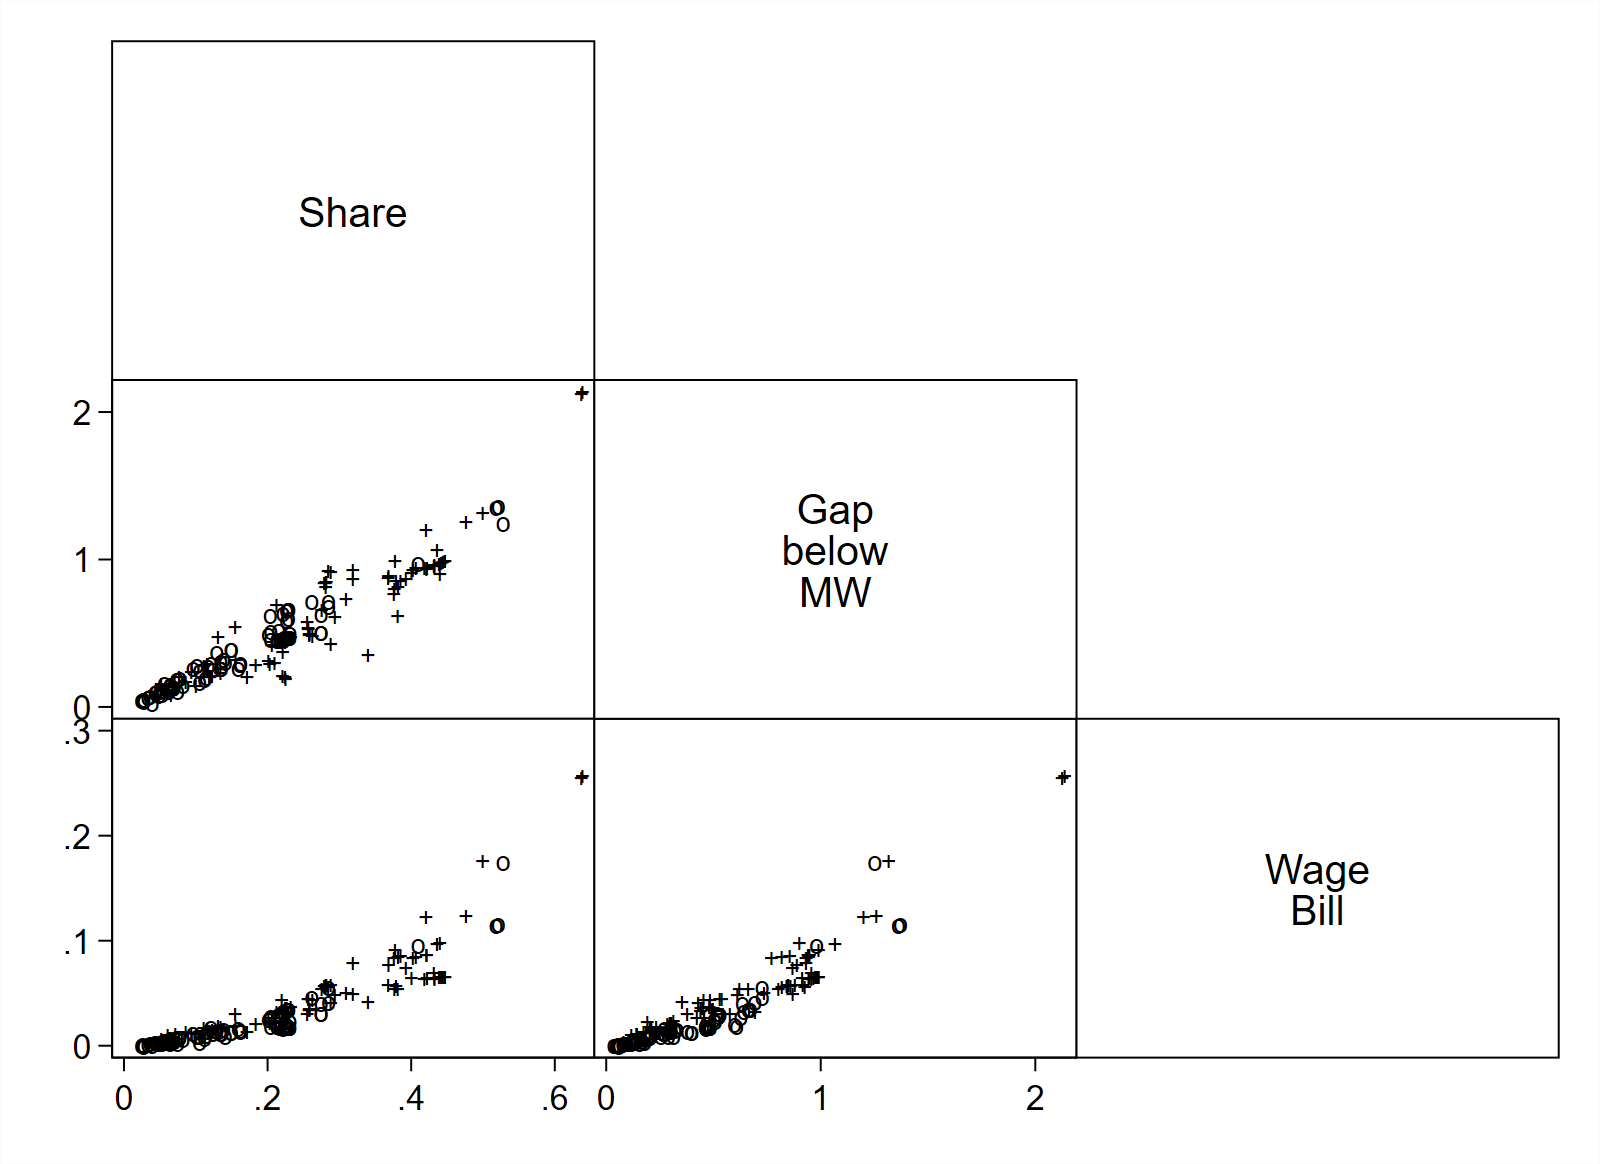
\includegraphics[width=0.70\paperwidth]{Images/shareGapWbi.png}
    \label{fig:correlationIndicators}
    \caption*{See notes below Table \ref{table:sectorBite} for a description of the indicators. +: values for sectors in the East, o: the West.}
\end{figure}

% Tw Results
% Replication: ctrl+F #twResultsTable
\begin{table}[htbp]\centering
\caption{Employment and Turnover Effects - Smaller Grey Zone}\label{table:twResults}
\begin{threeparttable}
\begin{tabular}{l|cc|cc}
\toprule
&\multicolumn{2}{c|}{East}&\multicolumn{2}{c}{West}\\
&Emp&Turn & Emp&Turn\\
&(1)&(2)&(3)&(4)\\
\midrule
$\Delta$ Growth 14-15 &-.002& 0& 0 & -.003\\
&(.002)& (.003)& (.002) & (.002) \\
$\Delta$ Growth 14-16 &-.006& 0& -.001 & -.005\\
&(.003)\sym{**}& (.004)& (.002) & (.003) \\
\midrule
\# of treated &7256& 5168& 12164 & 8688\\
\# of controls &66176& 47280& 66176 & 47281\\
\# of controls used &13328& 4730& 19250 & 7914\\
\midrule
SDM 13-14 &.03& 0& .01& -.01\\  % Note: East-Emp 1314 SDM exceeds point estimate SDM 
Level Diff 2013&0& -.01& 0& 0\\
Trend 2011-2014&\checkmark&\checkmark&\checkmark&\checkmark \\
Specification & Base & Prod & Base & Base\\
\bottomrule
\end{tabular}
\begin{tablenotes}
\item $\Delta$ Growth is the difference in growth between the treated and control. SDM refers to the standardised difference in means. 
Level Diff 2013 indicates the difference in log levels between treated and control in 2013. 
Trend indicates how this level difference evolved between 2011 and 2014.
Specification shows which matching specification scored best at the evaluation criteria. Prod: match also on 2014 labour productivity of firm (emp/turn).
\item Matching uncertainty robust AI standard errors in parentheses \citep{Abadie2006}.
\item \emph{Stars}: \sym{*} \(p<0.1\), \sym{**} \(p<0.05\), \sym{***} \(p<0.01\)
\end{tablenotes}
\end{threeparttable}
\end{table}


\end{document}

